\documentclass{article}
\usepackage{tikz}
\usetikzlibrary{arrows.meta,positioning,calc,shapes.geometric}
\pagestyle{empty}
\begin{document}
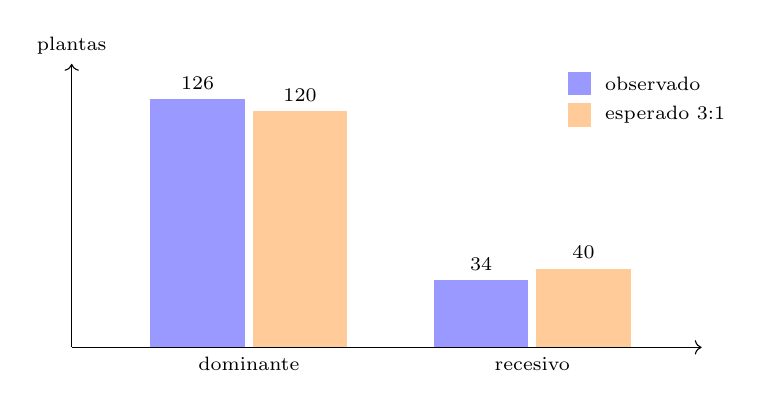
\begin{tikzpicture}

\draw[->] (0,0) -- (0,3.6) node[above, font=\scriptsize] {plantas}; \draw[->] (0,0) -- (8.0,0);
\foreach \x/\o/\e/\t in {1.0/126/120/dominante, 4.6/34/40/recesivo} {
  \fill[blue!40] (\x,0) rectangle (\x+1.2,{\o*0.025}); \fill[orange!40] (\x+1.3,0) rectangle (\x+2.5,{\e*0.025});
  \node[font=\scriptsize, above] at (\x+0.6,{\o*0.025}) {\o}; \node[font=\scriptsize, above] at (\x+1.9,{\e*0.025}) {\e}; \node[font=\scriptsize, below] at (\x+1.25,0) {\t};}
\fill[blue!40] (6.3,3.2) rectangle (6.6,3.5); \node[font=\scriptsize, right] at (6.65,3.35) {observado}; \fill[orange!40] (6.3,2.8) rectangle (6.6,3.1); \node[font=\scriptsize, right] at (6.65,2.95) {esperado 3:1};

\end{tikzpicture}
\end{document}
